\documentclass[11pt,a4paper]{article}
\usepackage[UTF8,fontset=none]{ctex}
\usepackage{fontspec}
\setmainfont{DejaVu Serif}
\setsansfont{DejaVu Sans}
\setCJKmainfont{Noto Serif CJK SC}
\setCJKsansfont{Noto Sans CJK SC}
\setCJKmonofont[Extension=.otf]{FandolFang-Regular}
\usepackage[a4paper,top=18mm,bottom=19mm,left=19mm,right=19mm]{geometry}
\usepackage{graphicx,booktabs,tabularx,array}
\graphicspath{{demo-assets/}}
\usepackage{amsmath,amssymb}
\usepackage{xcolor}
\usepackage{titlesec}
\usepackage{fancyhdr}
\usepackage{caption,subcaption}
\usepackage{float}
\usepackage{hyperref}
\usepackage[most]{tcolorbox}
\usepackage{microtype}
\usepackage{tikz}
\usepackage{listings}
% Smart Cities & Location Services — P2 Cloud Sorbet
% LOCKED visual palette v1 for Experiment Report
\definecolor{Paper}{HTML}{FCFAF7}
\definecolor{Ink}{HTML}{2D3238}
\definecolor{Muted}{HTML}{70757A}
\definecolor{P1}{HTML}{D3EAF5} % light blue
\definecolor{P2}{HTML}{F5D9B8} % apricot
\definecolor{P3}{HTML}{E8C7D3} % soft rose
\definecolor{P4}{HTML}{D7D3EA} % mist violet
\definecolor{C1}{HTML}{5B9FBE} % blue accent
\definecolor{C2}{HTML}{D49757} % apricot accent
\definecolor{C3}{HTML}{B97589} % rose accent
\definecolor{C4}{HTML}{8177A8} % violet accent
\definecolor{Rule}{HTML}{DDE3E7}
\definecolor{Panel}{HTML}{FFFDFC}

\pagecolor{Paper}\color{Ink}
\hypersetup{colorlinks=true,linkcolor=C1,urlcolor=C1,citecolor=C4}
\setlength{\parindent}{2em}\setlength{\parskip}{0.24em}\linespread{1.17}
\titleformat{\section}[hang]{\sffamily\bfseries}{\fontsize{26}{26}\selectfont\color{C1}\thesection}{0.68em}{\Large}
\titleformat{\subsection}{\sffamily\large\bfseries\color{Ink}}{\thesubsection}{0.55em}{}
\titlespacing*{\section}{0pt}{1.85em}{0.75em}
\pagestyle{fancy}\fancyhf{}
\fancyhead[L]{\sffamily\small\color{Muted}SMART CITIES \& LOCATION SERVICES}
\fancyhead[R]{\sffamily\small\color{Muted}Experiment Report}
\fancyfoot[C]{\sffamily\small\color{Muted}\thepage}
\renewcommand{\headrulewidth}{0pt}
\captionsetup{font=small,labelfont={bf,sf,color=Ink},textfont={color=Ink},skip=5pt}
\newtcolorbox{finding}{enhanced,boxrule=0pt,frame hidden,colback=P1!60!white,borderline west={2.4pt}{0pt}{C1},left=4mm,right=4mm,top=2.7mm,bottom=2.7mm,arc=0mm}
\newtcolorbox{noteBox}{enhanced,boxrule=.5pt,colframe=Rule,colback=P2!55!white,left=4mm,right=4mm,top=2.5mm,bottom=2.5mm,arc=1mm}
\newcommand{\metric}[3]{\begin{tcolorbox}[boxrule=0pt,colback=#1!55!white,arc=1.5mm,left=3mm,right=3mm,top=2.3mm,bottom=2.3mm]\sffamily\small\color{Muted}#2\\[-.4mm]{\Large\bfseries\color{Ink}#3}\end{tcolorbox}}
\lstset{basicstyle=\ttfamily\small,frame=single,rulecolor=\color{Rule},backgroundcolor=\color{Panel},breaklines=true,showstringspaces=false}
\begin{document}

% The unnumbered cover must not duplicate the following page.1 anchor.
\hypersetup{pageanchor=false}
\begin{titlepage}
\thispagestyle{empty}
\vspace*{25mm}
{\sffamily\small\color{C1}\bfseries SMART CITIES \& LOCATION SERVICES}\par
\vspace{5mm}
{\sffamily\fontsize{27}{32}\selectfont\bfseries Experiment Report}\par
\vspace{3mm}
{\Large 轨迹数据预处理与质量评估}\par
\vspace{12mm}
\noindent\color{Rule}\rule{\linewidth}{0.8pt}\color{Ink}
\vspace{10mm}
\begin{tabular}{@{}>{\sffamily\color{Muted}}p{28mm}p{100mm}@{}}
报告类型 & Experiment Report \\
视觉基线 & P2 · Cloud Sorbet \\
版式方向 & B · Visual Research + A · Minimal Cover \\
状态 & Design System Preview（合成示例数据）
\end{tabular}
\vfill
\noindent\color{P1}\rule{0.30\linewidth}{3.2pt}%
\color{P2}\rule{0.22\linewidth}{3.2pt}%
\color{P3}\rule{0.24\linewidth}{3.2pt}%
\color{P4}\rule{0.12\linewidth}{3.2pt}\par
\vspace{5mm}
{\small\color{Muted}此 PDF 用于冻结 Experiment Report 的视觉方向。所有数值和图均为模板合成示例，不属于实验一结果。}
\end{titlepage}
\hypersetup{pageanchor=true}

\tableofcontents\clearpage

\section{数据与问题}
\begin{finding}
\textbf{阅读入口。} 正式报告先用一句话说明最重要的数据问题，再给图和定量证据。这里的浅蓝信息块只承担章节级重点，不会每页重复出现。
\end{finding}

\vspace{0.5em}
\noindent\begin{minipage}[t]{0.32\linewidth}
\metric{P1}{轨迹数量}{11,386}\end{minipage}\hfill
\begin{minipage}[t]{0.32\linewidth}
\metric{P2}{轨迹点}{1.17 M}\end{minipage}\hfill
\begin{minipage}[t]{0.32\linewidth}
\metric{P3}{中位采样间隔}{10 s}\end{minipage}

\vspace{0.7em}
\begin{table}[H]
\centering
\caption{版式示例：基础统计用克制表格呈现，颜色只用于真正需要强调的信息。}
\begin{tabular}{lrrr}
\toprule
轨迹类型 & 数量 & 中位速度/(m/s) & 异常率/\% \\
\midrule
静止 & 126 & 0.12 & 0.8 \\
混合 & 34 & 0.78 & 2.6 \\
行驶 & 40 & 2.31 & 1.4 \\
\bottomrule
\end{tabular}
\end{table}

\section{方法如何改变空间轨迹}
\begin{figure}[H]
\centering
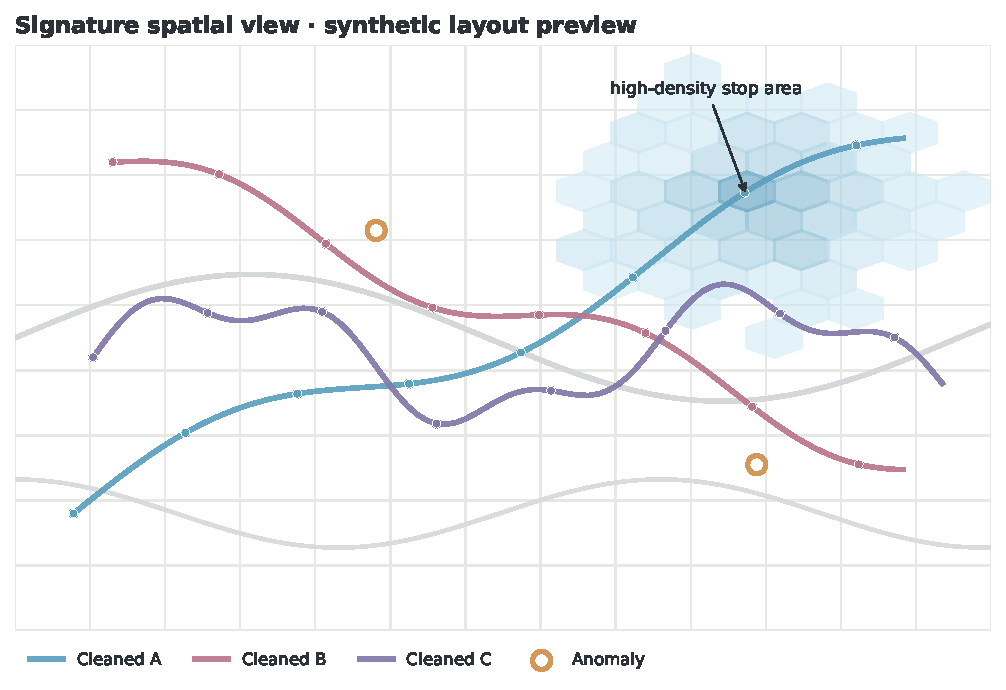
\includegraphics[width=0.99\linewidth]{signature_map.pdf}
\caption{Signature Visualization 示例。地图型主视觉同时承担空间上下文、轨迹结果、异常点、关键点和局部密度展示。}
\end{figure}

正式报告中，此类主图只在确实有空间意义时使用。底图应低饱和、数据为视觉主体，annotation直接指出需要老师注意的局部现象。

\section{参数与多目标权衡}
\begin{figure}[H]
\centering
\begin{subfigure}[t]{0.49\linewidth}
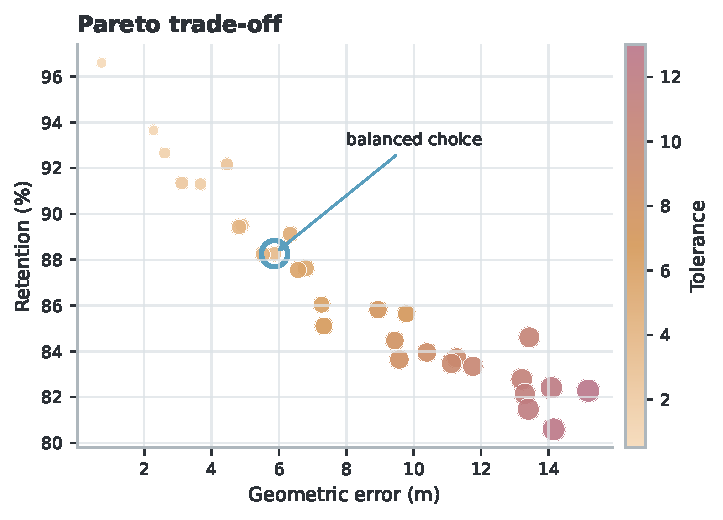
\includegraphics[width=\linewidth]{pareto.pdf}
\caption{误差—保留率—运行成本的联合编码}
\end{subfigure}\hfill
\begin{subfigure}[t]{0.49\linewidth}
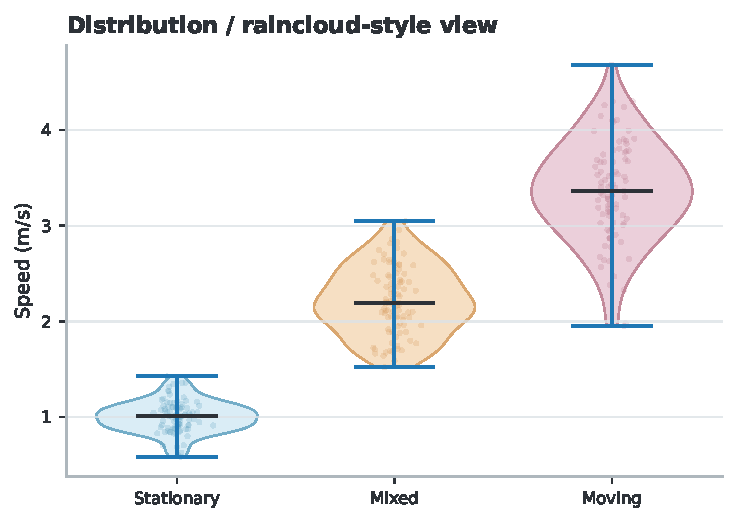
\includegraphics[width=\linewidth]{distribution.pdf}
\caption{不同轨迹类型的完整分布}
\end{subfigure}
\caption{多 Panel 示例：不同图承担互补信息，而不是机械重复同一个指标。}
\end{figure}

\begin{noteBox}
\textbf{版式原则。} 当一个参数不存在单一“最大最好”时，优先展示权衡关系和稳定区域，再在正文说明为什么选择最终方案；不只给一张柱状图宣布某个参数最好。
\end{noteBox}

\section{多指标方法比较}
\begin{figure}[H]
\centering
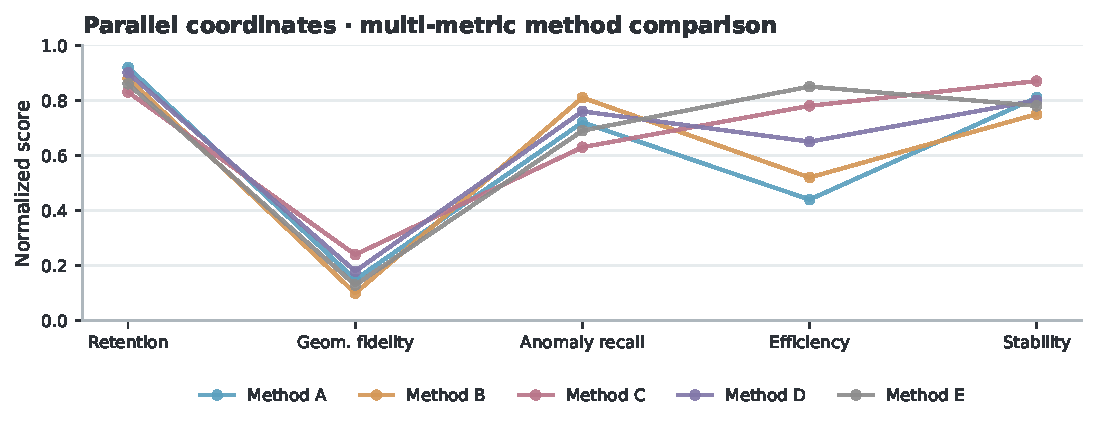
\includegraphics[width=0.96\linewidth]{parallel.pdf}
\caption{Parallel Coordinates 示例：在统一尺度上同时比较多个评价维度。}
\end{figure}

这类多维图适合展示“某个方法在多数指标上均衡，但并非每项绝对最高”的情况。颜色用于区分方法，线宽仅突出最终选择，不额外增加无意义视觉维度。

\section{参数敏感性与稳健区域}
\begin{figure}[H]
\centering
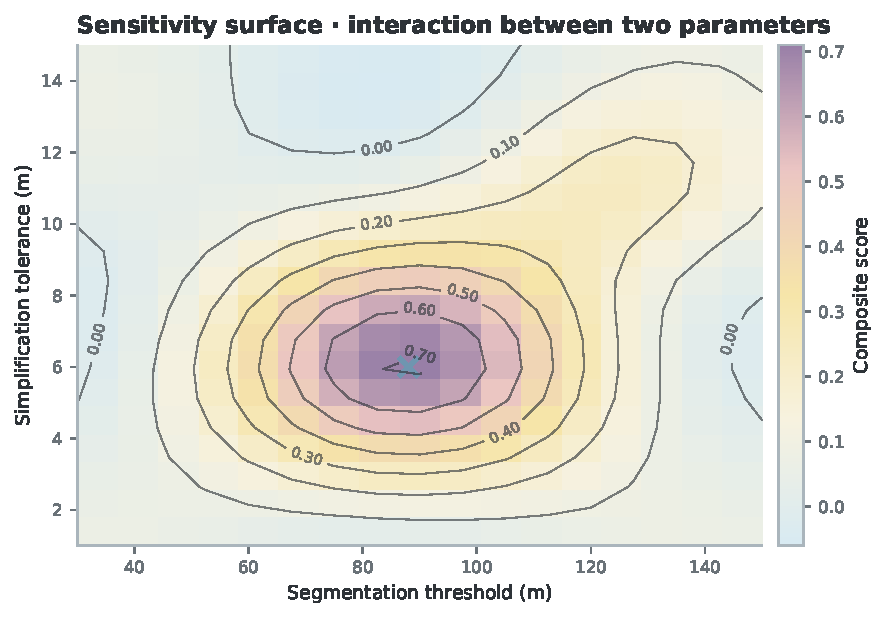
\includegraphics[width=0.80\linewidth]{sensitivity.pdf}
\caption{Heatmap + contour 示例：展示两个参数的联合作用以及相对稳定的高分区域。}
\end{figure}

\begin{finding}
\textbf{视觉目标。} P2 Cloud Sorbet 配色在正文中保持暖白、淡蓝、杏黄、柔粉和灰紫的柔和基调；数据图使用同色系中更深的描边和曲线，避免“淡色很好看，但科研图看不清”的问题。
\end{finding}

\section{技术批判与正式写作}
技术批判进入 Experiment Report 时应聚焦可验证的技术事实，例如单位、坐标、投影、插值假设和评价指标。完整聊天过程留在 Process Report。

\begin{lstlisting}[language=Python,caption={关键代码只展示有助于理解方法的部分}]
def evaluate_candidate(candidate, reference):
    # The report explains why these metrics are used.
    return retention, geometry_error, continuity
\end{lstlisting}

\section{当前模板方向}
这一版本只冻结视觉方向，不锁死具体章节名称。后续根据老师题目调整章节结构，但保持统一字体、P2配色、图注、表格、页眉页脚、Panel间距和图表风格。

\end{document}
